
\chapter{Documentación de HARDroid}
\label{index:har-index}\label{index:hardroid}\label{index:human-activity-recognition-for-android}

\section{Acerca de HARDroid}
\label{index:bienvenido-a-la-documentacion-de-hardroid}
Este proyecto es un servicio de reconocimiento de actividades humanas
para Android. Utiliza dos componentes de librería y un APK de servicio
para reutilizar el código.

Puedes ver el abance del proyecto en el repositorio \href{https://github.com/hardroidpy}{GitHub}  y
verificar la documentación JavaDoc para saber más detalles del
funcionamiento de la {\hyperref[glossary:term\string-api]{\termref{\DUrole{xref,std,std-term}{API}}}}.


\subsection{Autores}
\label{index:autores}\begin{itemize}
\item {} 
\href{https://github.com/agimenezpy}{Alberto G.}

\item {} 
\href{https://github.com/syegros}{Santiago Y.}

\end{itemize}
\phantomsection\label{index:har-content}

\subsection{¿Qué es HARDroid?}
\label{intro:har-intro}\label{intro::doc}\label{intro:que-es-hardroid}

\subsubsection{HARDroid}
\label{intro:hardroid}
\abbr{HARDroid} es un proyecto \emph{Open Source} que tiene como objetivo tener una implementación abierta del servicio de
reconocimiento de actividades físicas utilizando sensores del celular.

Nuestro proyecto implementa el concepto de desacomplamiento de una Librería \abbr{API} y una \abbr{APK} de servicio que provee la
funcionalidad de reconocimiento de actividades físicas.

La idea nace de dos productos similares de Google y Sony que realizan reconocimiento de actividades los cuales son
\emph{Google Play Services} y \emph{Sony LifeLog}.


\subsubsection{Google Play Services}
\label{intro:har-google-play-services}\label{intro:google-play-services}
Google dispone del producto Google Play Services \cite{Google2016ps}
que proporciona dentro de una \abbr{APK} la implementación de algoritmos, y además los desarrolladores de aplicaciones
Android pueden integrarse (a través de una \abbr{API} \cite{Google2016l}) a varias
funcionalidades utilitarias en las siguientes dimensiones:
\begin{quote}
\begin{description}
\item[{Location \& Context}] \leavevmode
Provee funcionalidades para mejorar la precisión y calidad de la ubicación GPS del celular basado en sensores.
Además, la función \emph{contexto} provee la capacidad de reconocer las actividades físicas

\item[{Ads}] \leavevmode
Provee funcionalidades para ofrecer publicidad in la aplicación

\item[{Games}] \leavevmode
Provee funcionalidades para Gamificar la aplicación

\item[{Cloud Messaging}] \leavevmode
Provee funcionalidades para mensajería a travéz de Internet.

\end{description}


\end{quote}

\subsubsection{Sony LifeLog}
\label{intro:sony-lifelog}\label{intro:har-life-log}
Sony dispone de un producto registrar las actividades diarias de las personas por medio de sensores
del celular o por medio de las relojes \emph{smartwatch}. Para esto proveen una aplicación de rastreo de actividades
diarias con un reconocedor de actividades propio.
\begin{table}[!htbp]
\begin{tabular}{lll}
\textsf{\relax 
Inicio LifeLog
} & \textsf{\relax 
Configuración
} & \textsf{\relax 
Acerca del Reconocedor
}\\
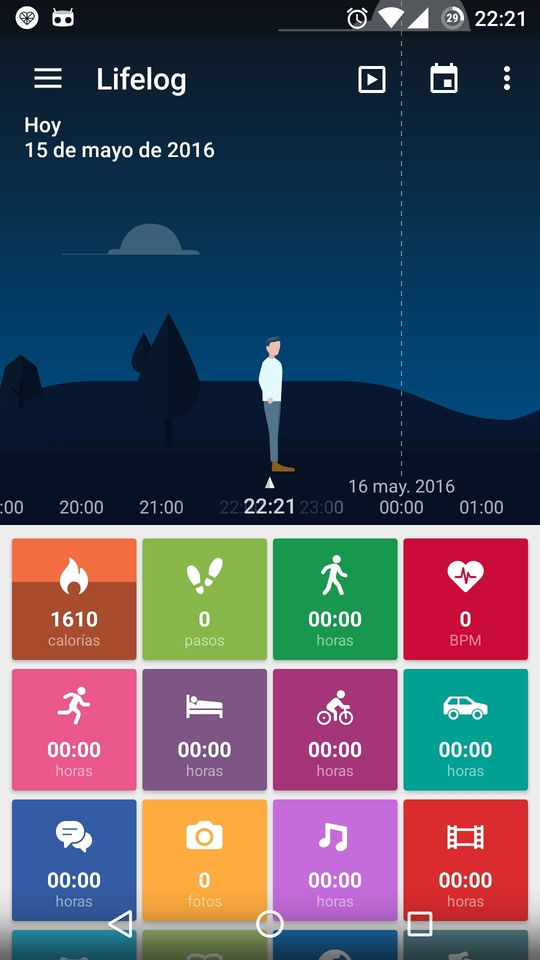
\includegraphics[width=0.33\textwidth]{anexos/graphics/lf_start.jpg}
 & 
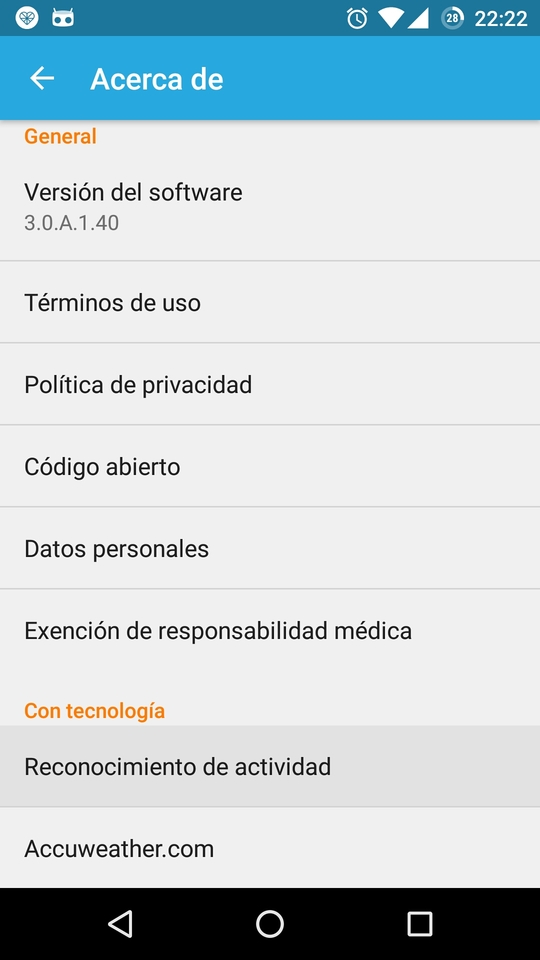
\includegraphics[width=0.33\textwidth]{anexos/graphics/lf_conf.jpg}
 & 
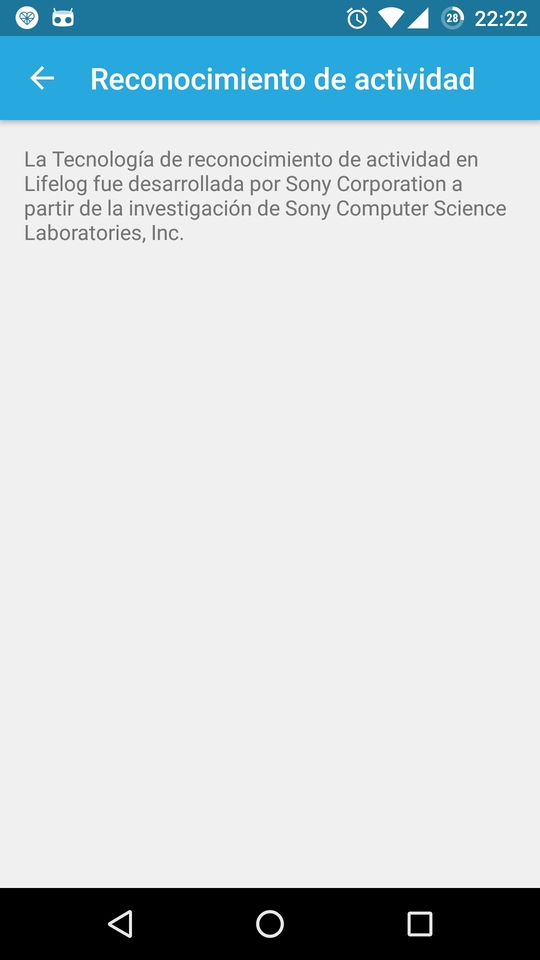
\includegraphics[width=0.33\textwidth]{anexos/graphics/lf_actrec.jpg}
\\
\end{tabular}
\end{table}

\section{Primeros Pasos}
\label{first:har-first}\label{first::doc}\label{first:primeros-pasos}

\subsubsection{Instalar las Aplicaciones}
\label{first:instalar-las-aplicaciones}
El proyecto se compone de dos aplicaciones \emph{\abbr{Android}} que se comunican por medio de el protocolo \emph{BINDER} \abbr{IPC} de manera a
independizar las funciones de encuesta y servicio de reconocimiento.


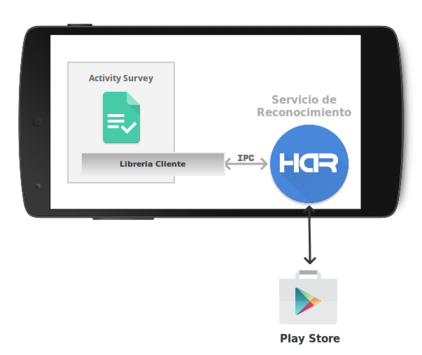
\includegraphics[width=0.7\textwidth]{anexos/graphics/archi_ipc.png}

Para contribuir con la recolección de datos sigue los pasos para instalar en tu celular las aplicaciones.

\paragraph{Instalar la Encuesta}
\label{first:instalar-la-encuesta}\label{first:har-survey}
Para instalar la aplicación \emph{Activity Survey} de encuesta accede a este URL \url{https://goo.gl/JHNL1B} o por medio de la siguiente
imagen:
\begin{figure}[!htbp]
   \centering
   
\includegraphics{anexos/graphics/qr_url.jpg}
\caption{Acceso al instalador \emph{Activity Survey}}\label{first:id1}\end{figure}

Descarga la aplicación desde
\emph{Google Play Store} \cite{GimenezYegros2016e}.
\begin{figure}[!htbp]
    \centering 
    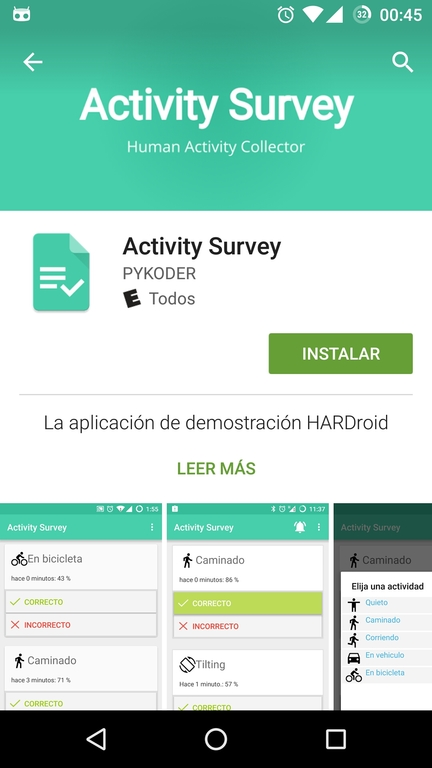
\includegraphics[width=0.4\textwidth]{anexos/graphics/inst_app5.jpg}
\caption{Instalador desde Google Play}\label{first:id2}\end{figure}

Si queres registrarte como un \emph{beta tester} registrate con tu cuenta de Google en \url{https://goo.gl/GjmMl3}.

\begin{table}[!htbp]
\begin{tabular}{lll}
\textsf{\relax 
Ingresar el URL
} & \textsf{\relax 
Logearse a Google
} & \textsf{\relax 
Aceptar ser tester
}\\
    {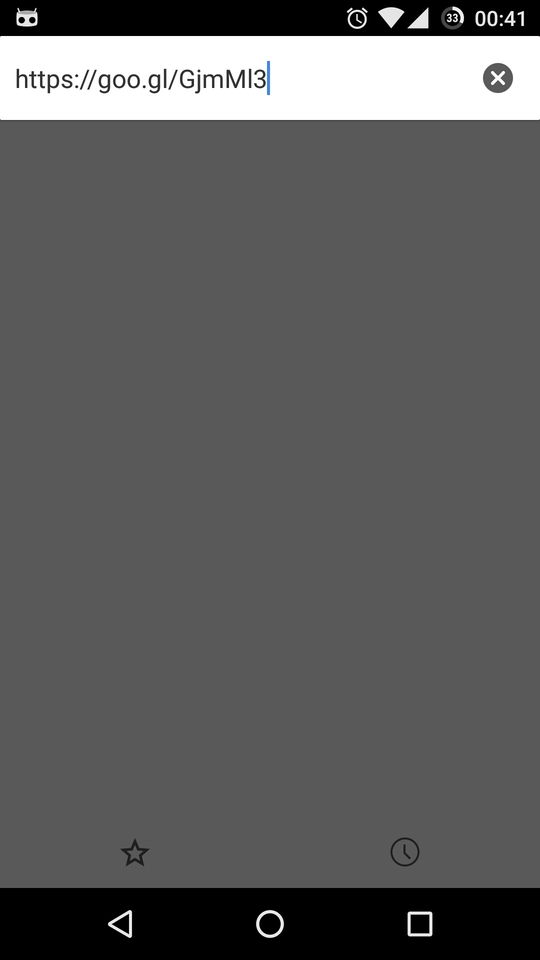
\includegraphics[width=0.33\textwidth]{anexos/graphics/inst_app.jpg}}
 & 
    {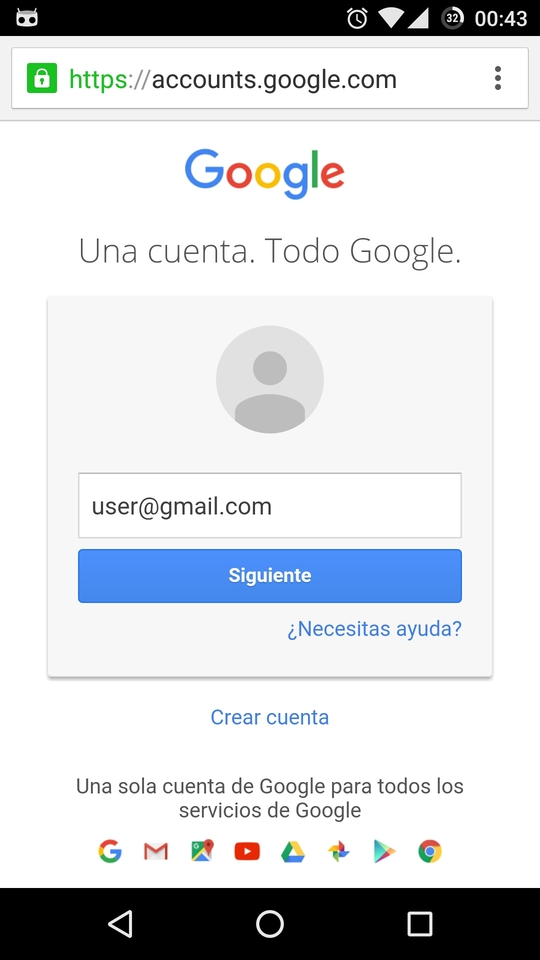
\includegraphics[width=0.33\textwidth]{anexos/graphics/inst_app2.jpg}}
 & 
    {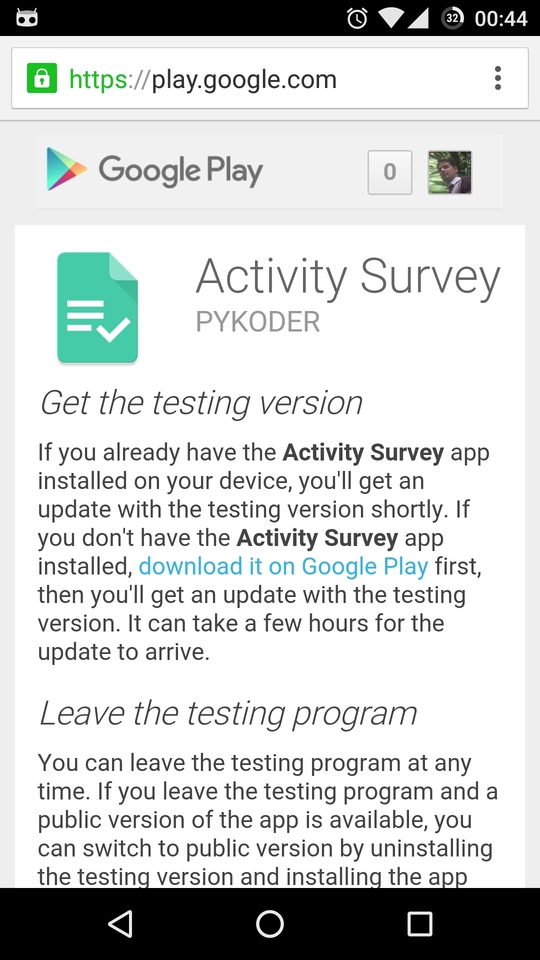
\includegraphics[width=0.33\textwidth]{anexos/graphics/inst_app4.jpg}}
\\
\end{tabular}
\end{table}


Para finalizar debes configurar la aplicación siguiendo los pasos en \hyperref[config:har-config]{Configurar Activity Survey}.


\paragraph{Instalar el Reconocedor}
\label{first:instalar-el-reconocedor}
Luego de instalar y configurar la aplicación de encuesta \emph{Activity Survey} (vease {\hyperref[config:har-config]{Configurar Activity Survey}),
al intentar utilizar el servicio este te pedira instalar del \emph{Google Play Store} el servicio reconocedor \emph{HARDroid}.

\begin{table}[h]
\begin{tabular}{ll}
\textsf{\relax 
Sugerencia para HARDroid
} & \textsf{\relax 
Instalar del Play Store
}\\
    {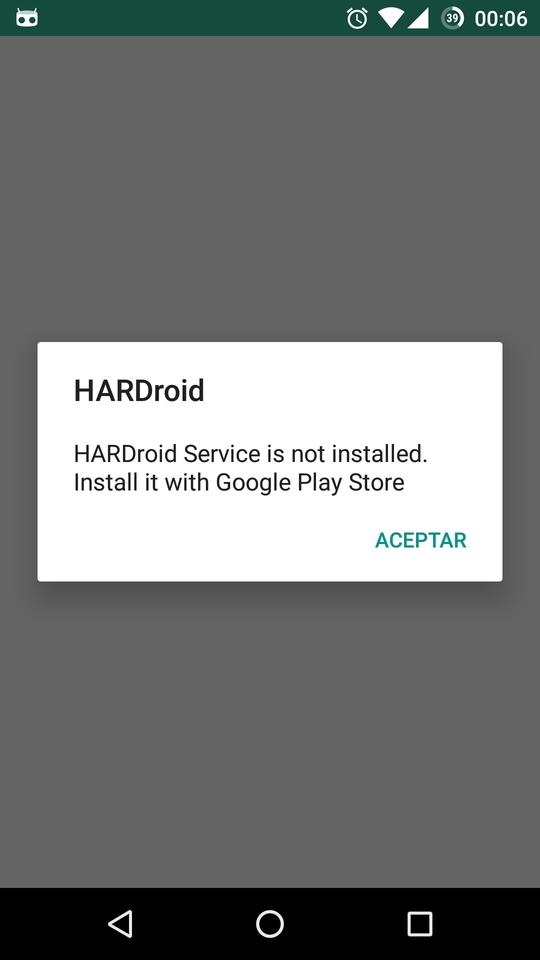
\includegraphics[width=0.33\textwidth]{anexos/graphics/install_service.jpg}}
 & 
    {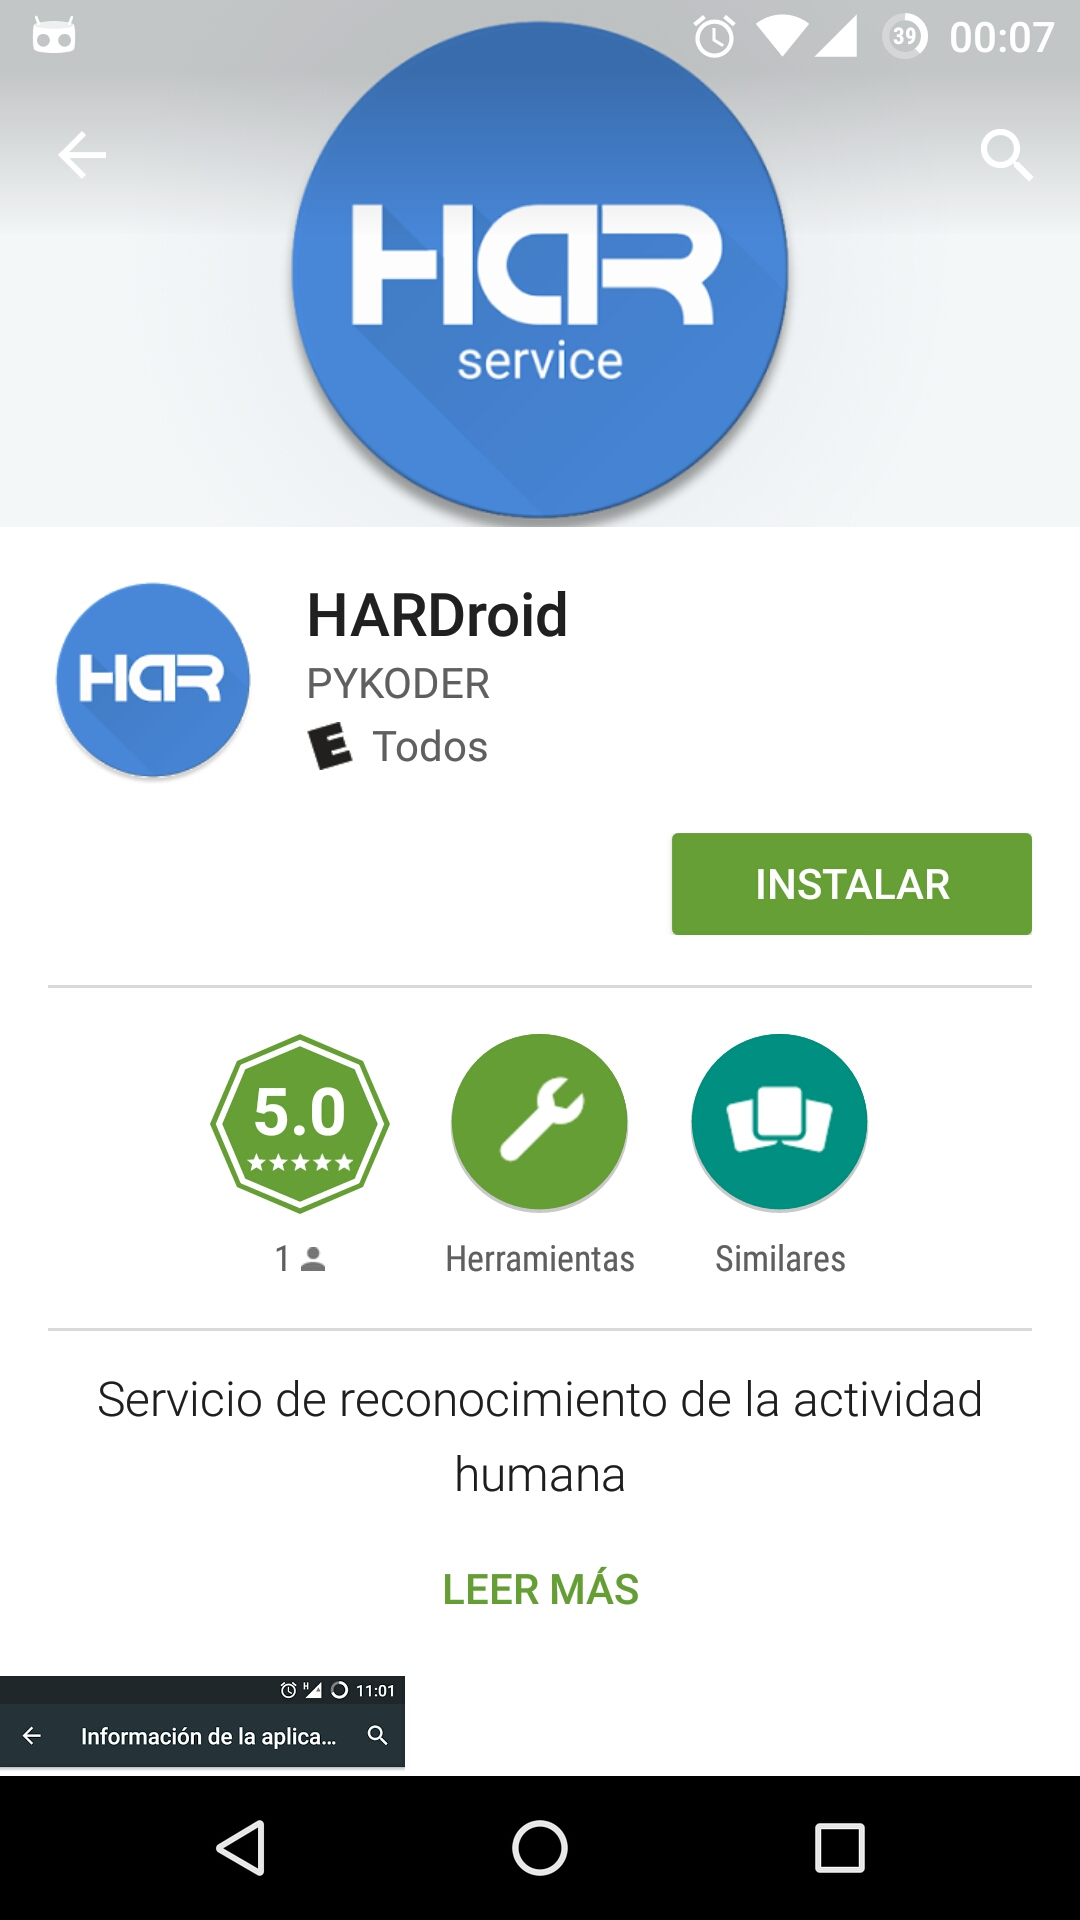
\includegraphics[width=0.33\textwidth]{anexos/graphics/inst_servplay.jpg}}
\\
\end{tabular}
\end{table}

\subsection{Configurar \emph{Activity Survey}}
\label{config:configurar-activity-survey}\label{config:har-config}\label{config::doc}

\subsubsection{Iniciar la encuesta}
\label{config:iniciar-la-encuesta}
Una vez instalada la aplicación de encuesta debes configurarla con los datos mínimos para iniciar
contribuir con la recolección.

Inicia la aplicación
\begin{figure}[h]
\centering
    {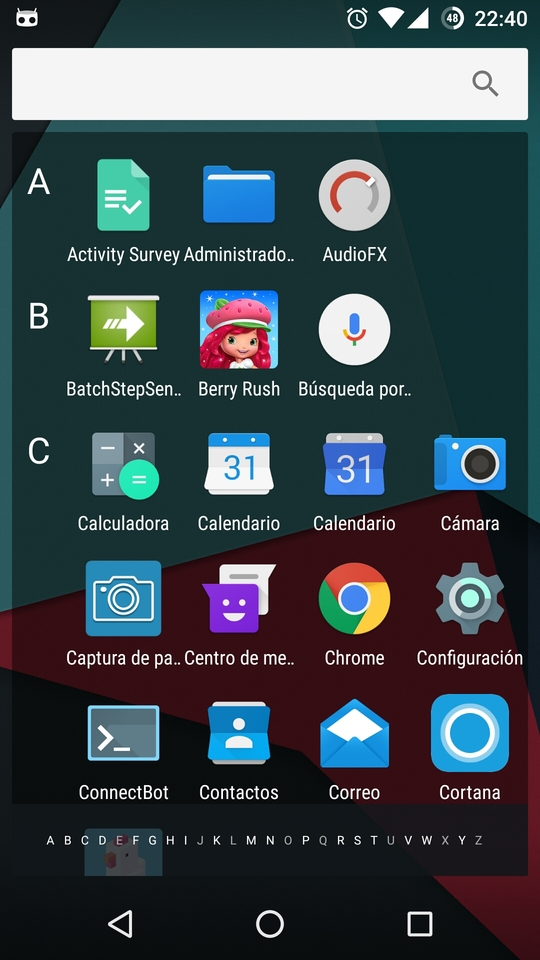
\includegraphics[width=0.4\textwidth]{anexos/graphics/app_inst.jpg}}
\caption{\emph{Activity Survey} instalada}\label{config:id1}\end{figure}

Lee las instrucciones y concede los permisos

\begin{table}[h]
\begin{tabular}{lll}
\textsf{\relax 
Iniciar la Encuesta
} & \textsf{\relax 
Aceptar y configurar
} & \textsf{\relax 
Dar permisos
}\\
    {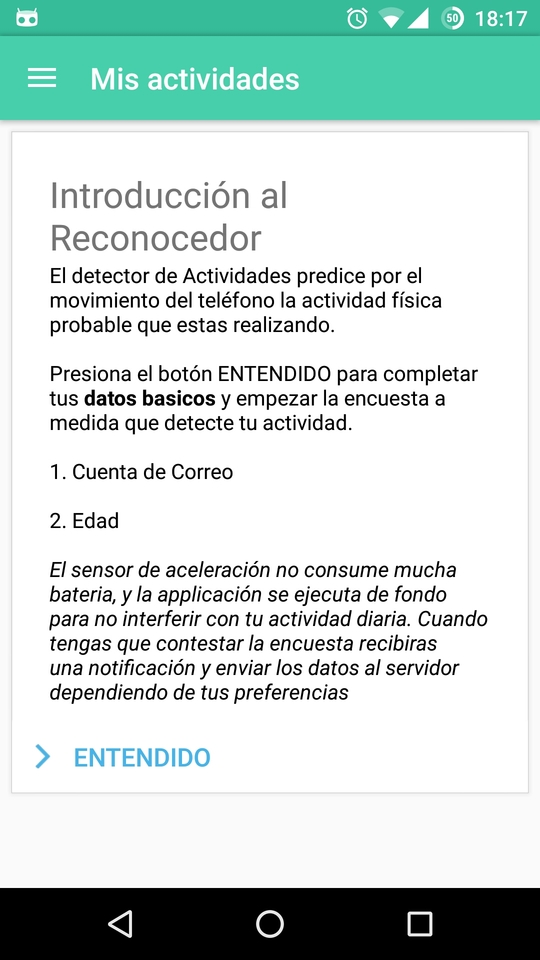
\includegraphics[width=0.33\textwidth]{anexos/graphics/app_start.jpg}}
 & 
    {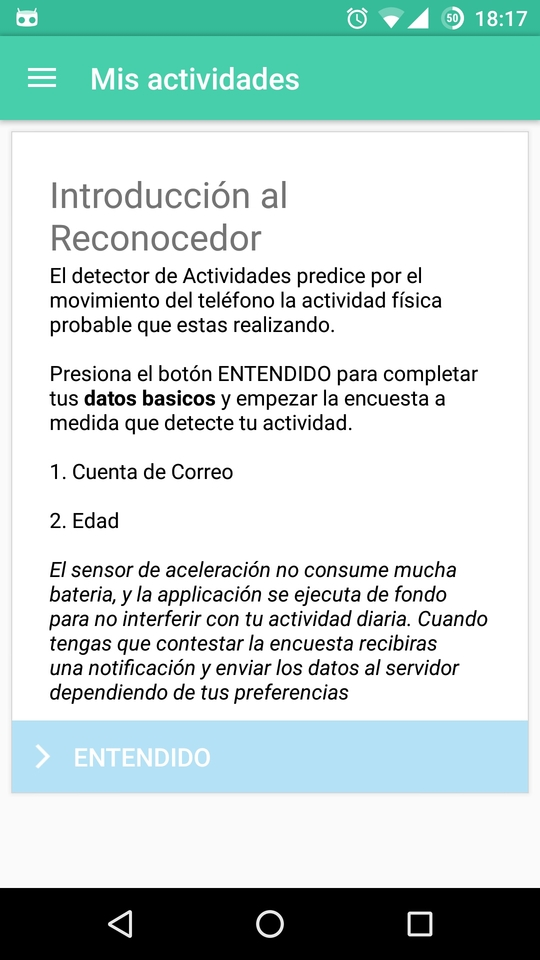
\includegraphics[width=0.33\textwidth]{anexos/graphics/app_start2.jpg}}
 & 
    {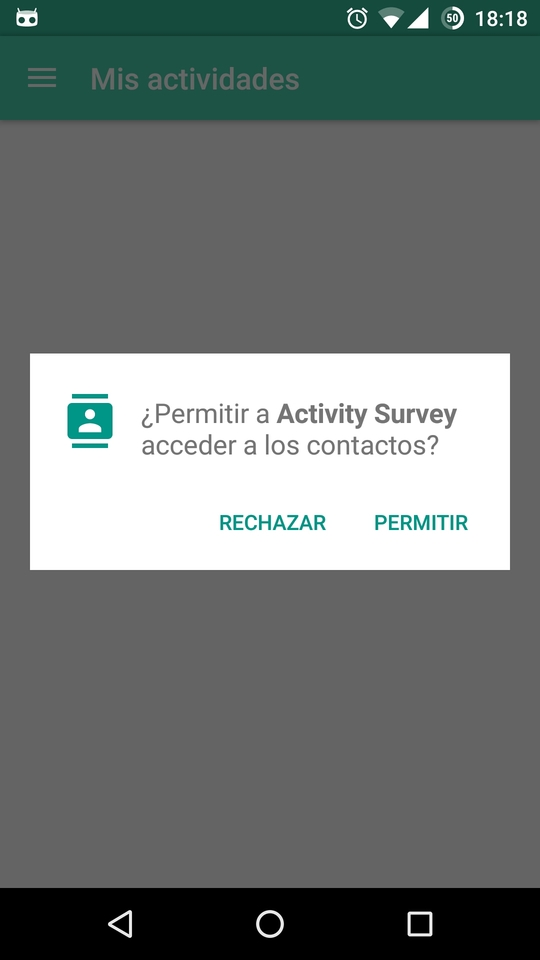
\includegraphics[width=0.33\textwidth]{anexos/graphics/app_perm.jpg}}
\\
\end{tabular}
\end{table}

\subsubsection{Ingresa tu correo y edad}
\label{config:ingresa-tu-correo-y-edad}
Para poder identificar tus contribuciones requerimos de datos mínimos para la encuesta.
\begin{figure}[h]
\centering
    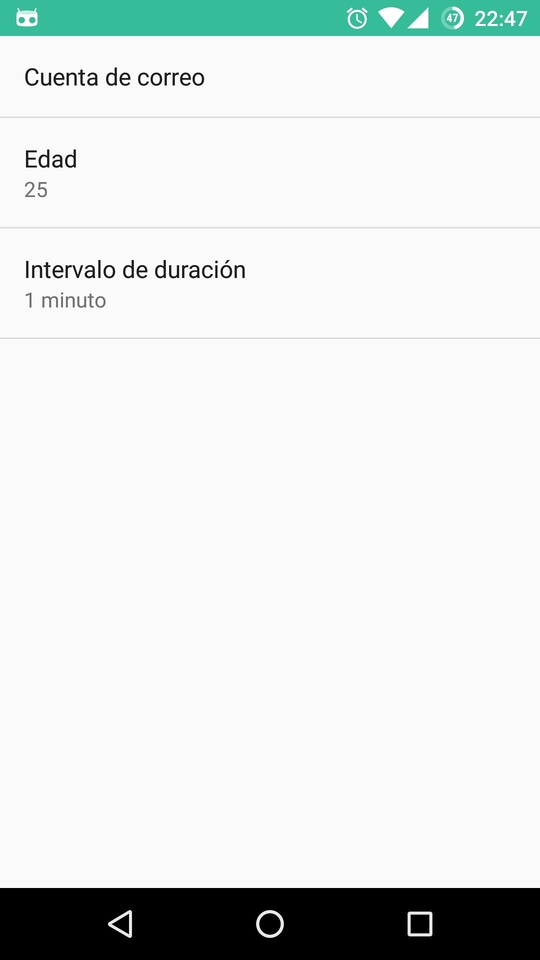
\includegraphics[width=0.4\textwidth]{anexos/graphics/app_conf.jpg}
\caption{Iniciar la configuración}\label{config:id2}\end{figure}

Configura los datos requeridos.
\begin{table}[h]
\begin{tabular}{lll}
\textsf{\relax 
Ingresa tu correo
} & \textsf{\relax 
Ingresa tu edad
} & \textsf{\relax 
Ingresa el intervalo
}\\
    {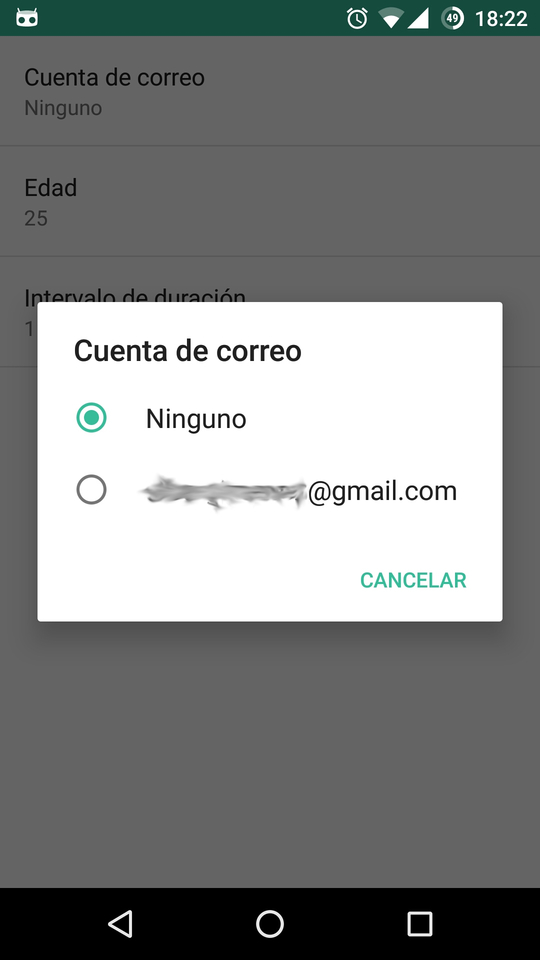
\includegraphics[width=0.33\textwidth]{anexos/graphics/app_email.jpg}}
 & 
    {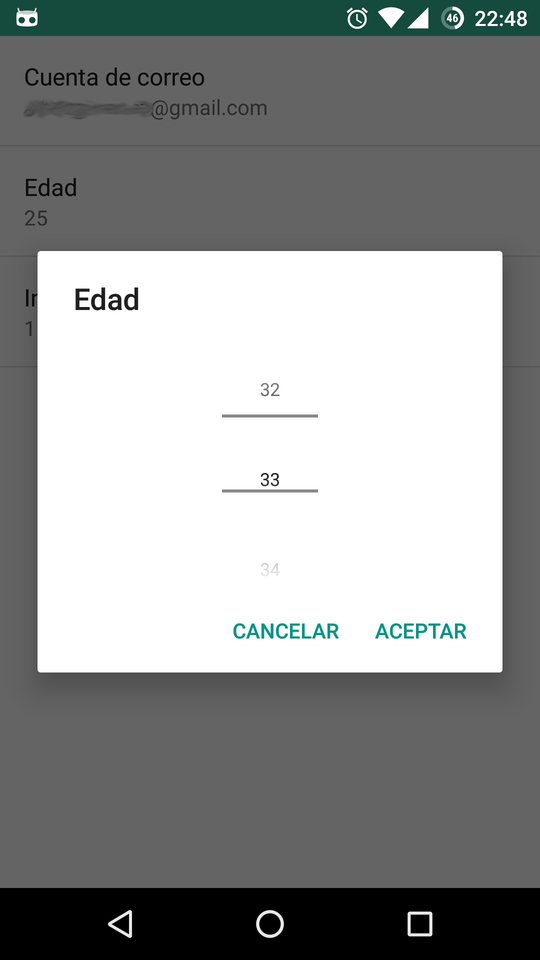
\includegraphics[width=0.33\textwidth]{anexos/graphics/app_age.jpg}}
 & 
    {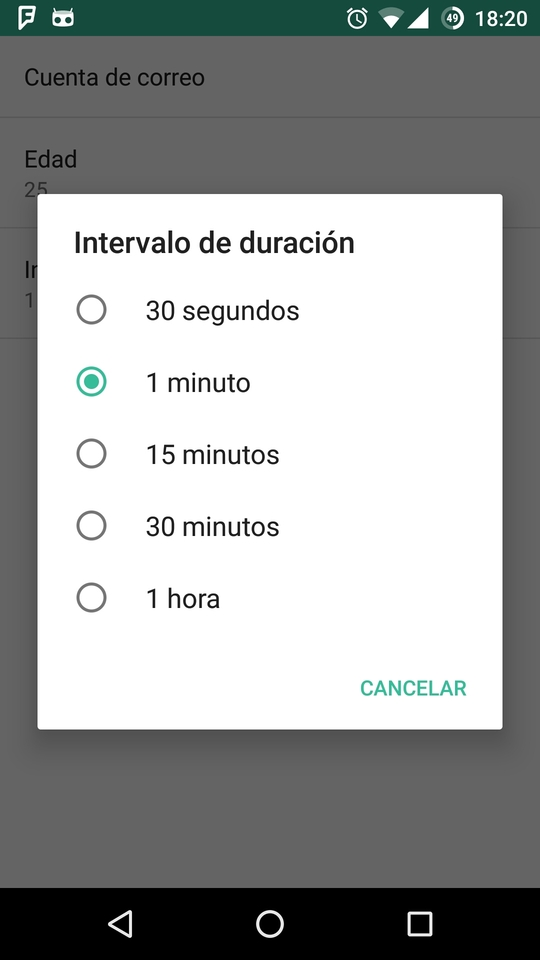
\includegraphics[width=0.33\textwidth]{anexos/graphics/app_int.jpg}}
\\
\end{tabular}
\end{table}


El servicio de reconocimiento se activará a cada minuto que eliga en la configuración:
\begin{itemize}
\item {} 
1 minuto

\item {} 
15 minutos

\item {} 
30 minutos

\item {} 
1 hora

\end{itemize}

\subsubsection{Servicio de Reconocimiento Activado}
\label{config:servicio-de-reconocimiento-activado}
Una vez configurado la aplicación de encuesta se conectará automáticamente al servicio de reconocimiento instalado.
\begin{figure}[h]
\centering

    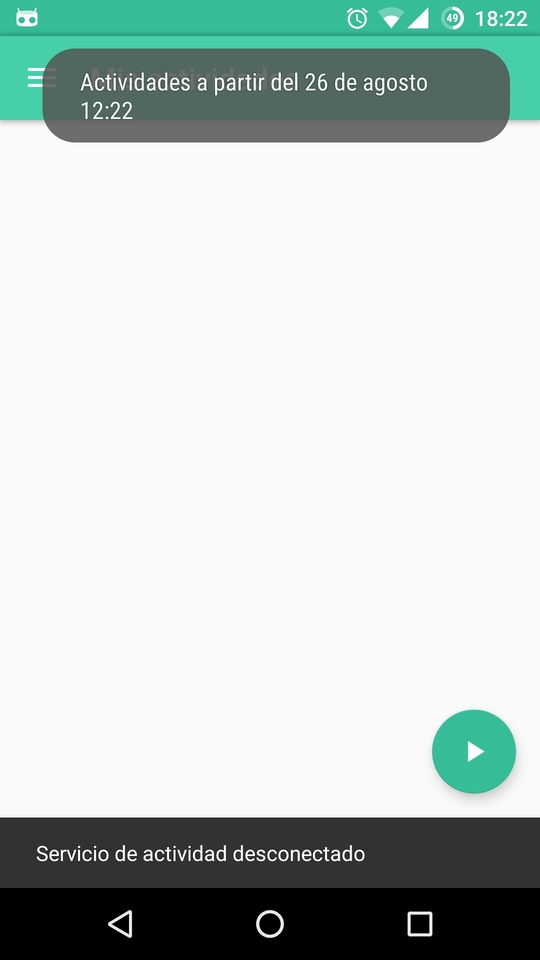
\includegraphics[width=0.4\textwidth]{anexos/graphics/app_started.jpg}
\caption{Servicio de Reconocimiento Iniciado}\label{config:id3}\end{figure}


\subsection{Contribuir con \emph{Activity Survey}}
\label{contrib:har-contrib}\label{contrib::doc}\label{contrib:contribuir-con-activity-survey}

\subsubsection{Ver tus actividades}
\label{contrib:ver-tus-actividades}
Dependiendo del intervalo de reconocimiento la aplicación desplegará las últimas 5 actividades recientes
reconocidas.

\begin{table}[h]
\begin{tabular}{ll}
\textsf{\relax 
Actividades recientes
} & \textsf{\relax 
Mas actividades
}\\
    {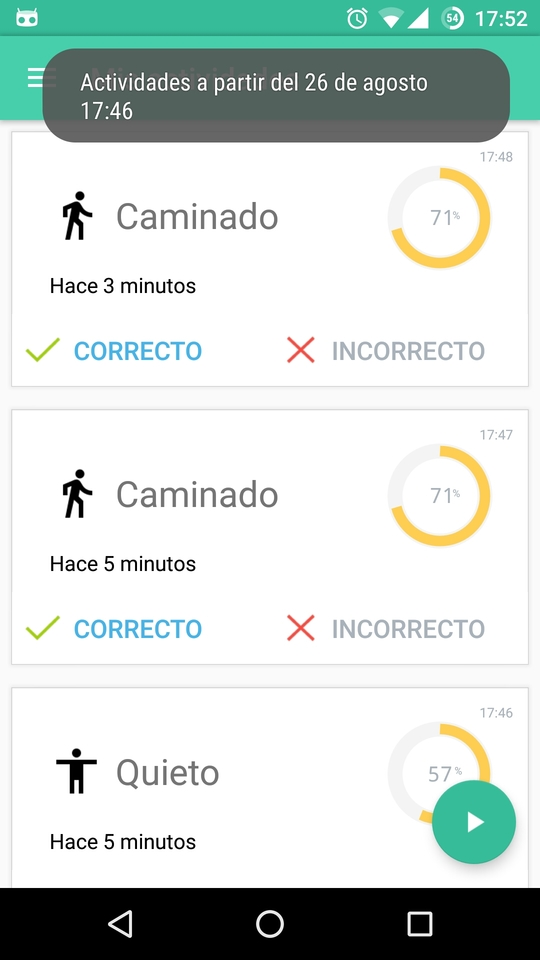
\includegraphics[width=0.33\textwidth]{anexos/graphics/activities_toast.jpg}}
 & 
    {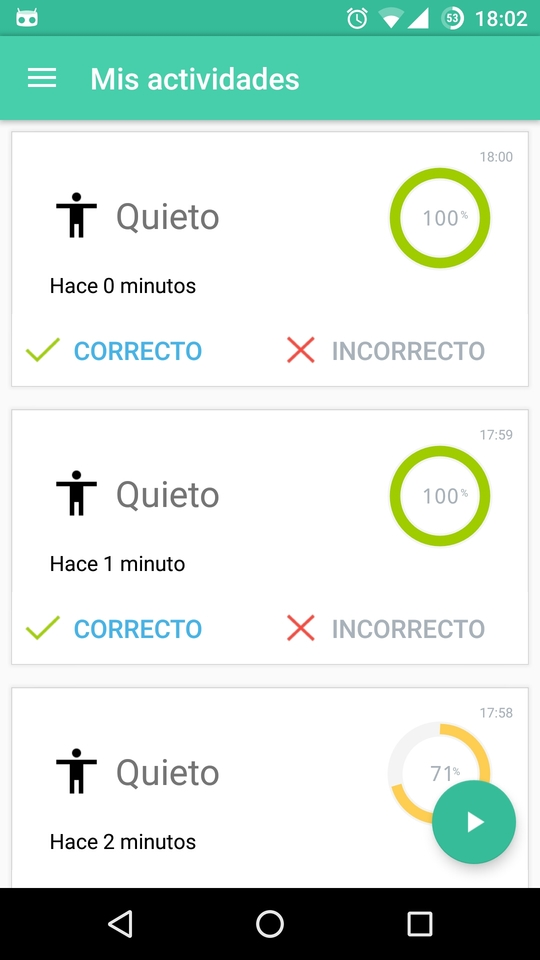
\includegraphics[width=0.33\textwidth]{anexos/graphics/activities.jpg}}
\\
\end{tabular}
\end{table}


Además recibiras notificaciones periodicas a medida que se reconozca una actividad.

\begin{table}[h]
\begin{tabular}{ll}
\textsf{\relax 
Notificación Recibida
} & \textsf{\relax 
Detalle de actividad
}\\
    {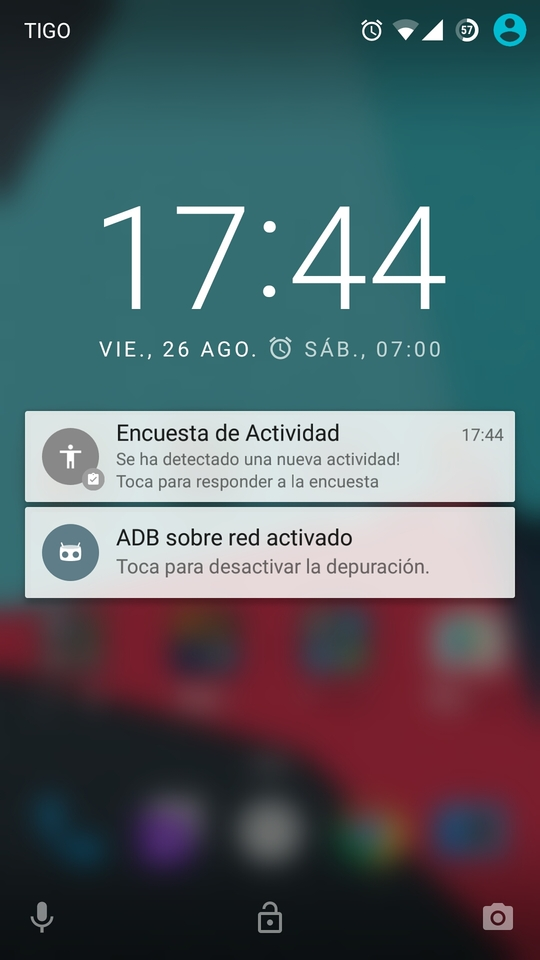
\includegraphics[width=0.33\textwidth]{anexos/graphics/scr_notification.jpg}}
 & 
    {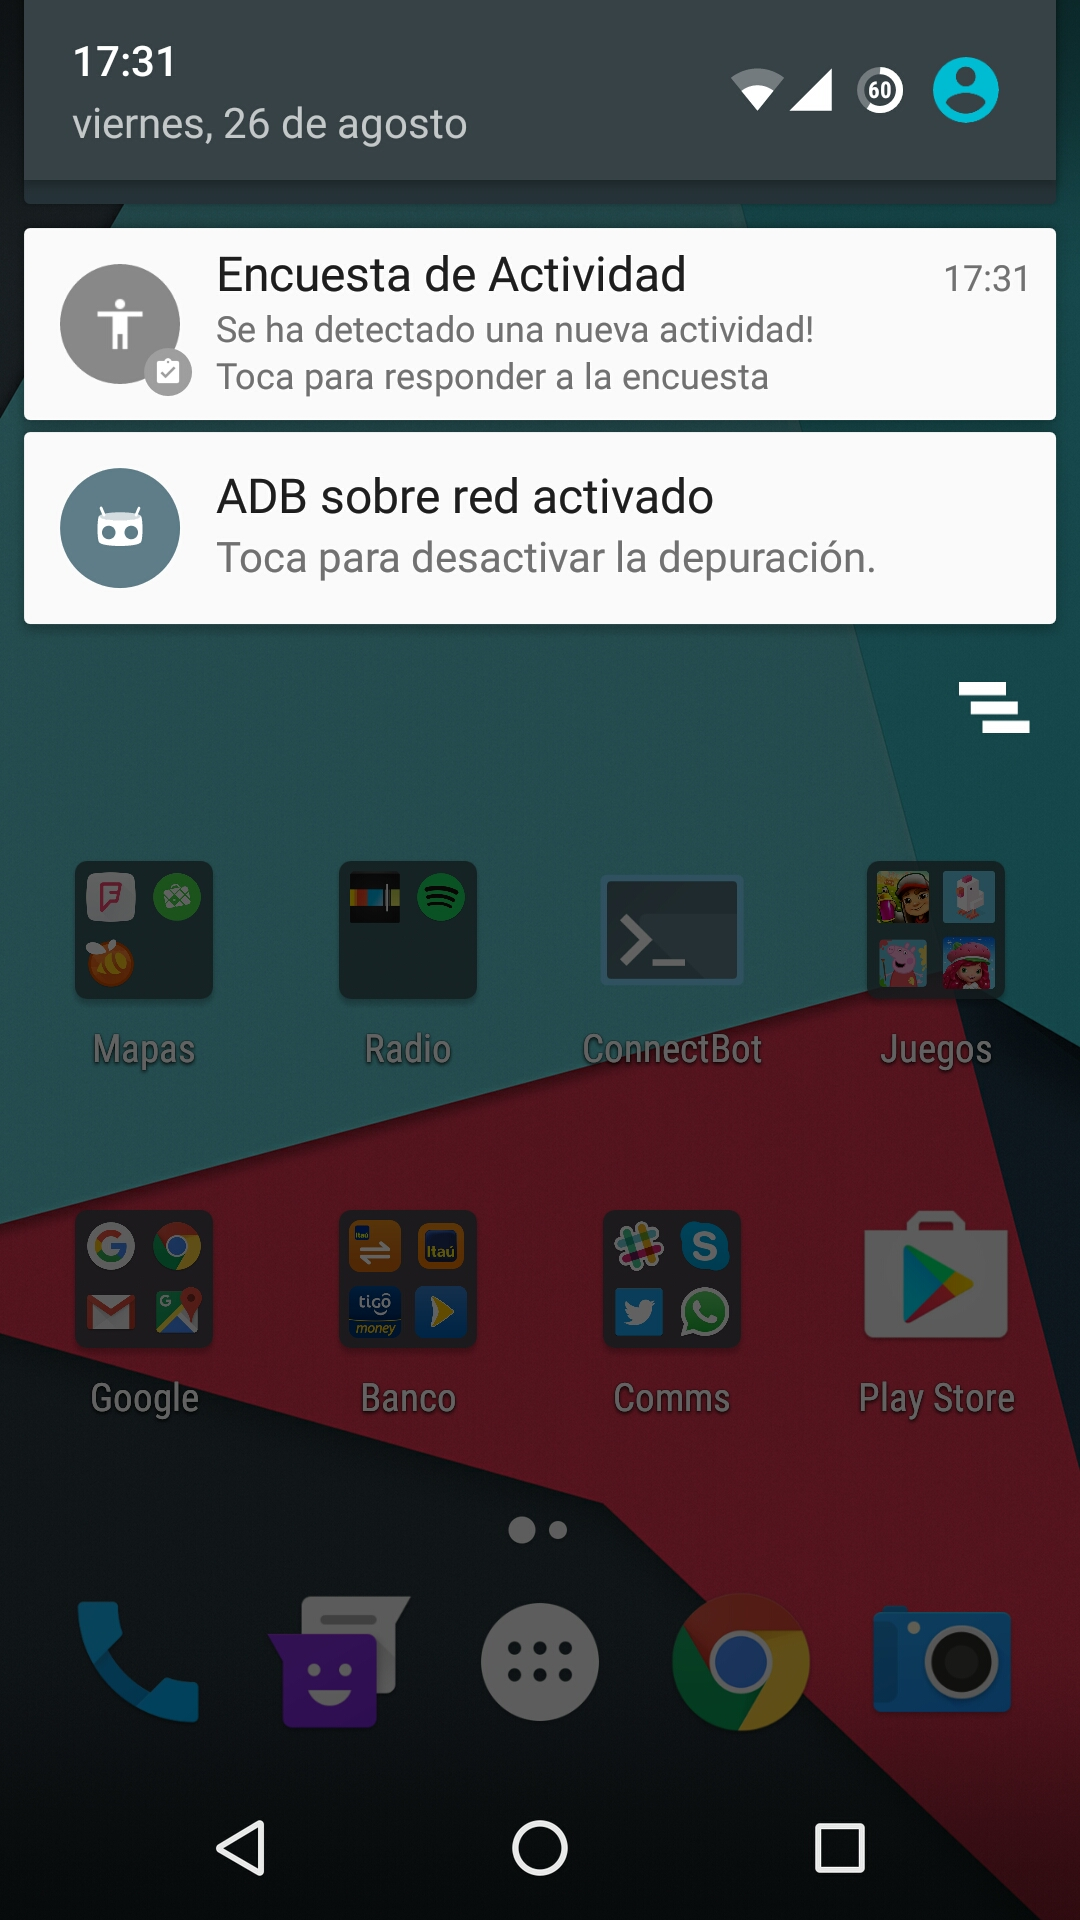
\includegraphics[width=0.33\textwidth]{anexos/graphics/bar_notification2.jpg}}
\\
\end{tabular}
\end{table}



\subsubsection{Actividades Conocidas}
\label{contrib:actividades-conocidas}
Las actividades que el servicio reconoce son:
\begin{quote}
\begin{description}
\item[{Quieto}] \leavevmode
El servicio detectó que el teléfono móvil está quieto.


\includegraphics{anexos/graphics/still.png}

\item[{Caminando}] \leavevmode
El servicio detectó que el teléfono móvil está en movimiento lento.


\includegraphics{anexos/graphics/walk.png}

\item[{Correr}] \leavevmode
El servicio detectó que el teléfono móvil está en movimiento apresurado.


\includegraphics{anexos/graphics/run.png}

\item[{En vehiculo}] \leavevmode
El servicio detectó que el teléfono móvil está en movimiento dentro de un vehiculo.


\includegraphics{anexos/graphics/car.png}

\item[{En bicicleta}] \leavevmode
El servicio detectó que el teléfono móvil está en movimiento sobre una bicicleta.


\includegraphics{anexos/graphics/bike.png}

\item[{Tilting}] \leavevmode
El servicio detectó que el teléfono móvil está girando.


\includegraphics{anexos/graphics/tilt.png}

\item[{Desconocido}] \leavevmode
El servicio no pudo detectar la actividad.


\includegraphics{anexos/graphics/unk.png}

\end{description}
\end{quote}

\subsubsection{Responder a la Encuesta}
\label{contrib:responder-a-la-encuesta}
Para responder a la encuesta tienes las siguientes opciones.
\begin{quote}
\begin{description}
\item[{Actividad Correcta}] \leavevmode
El servicio detecto correctamente la actividad física, marcarla como correcta (1)

\item[{Actividad Incorrecta}] \leavevmode
El servicio detectó incorrectamente la actividad física, marcala como incorrecta (2)
y proveer una retroalimentación con la actividad adecuada (3).

\end{description}
\end{quote}

\begin{table}[!htbp]
\begin{tabular}{lll}
\textsf{\relax 
Marcar correcto (1)
} & \textsf{\relax 
Marcar incorrecto (2)
} & \textsf{\relax 
Responder (3)
}\\
    {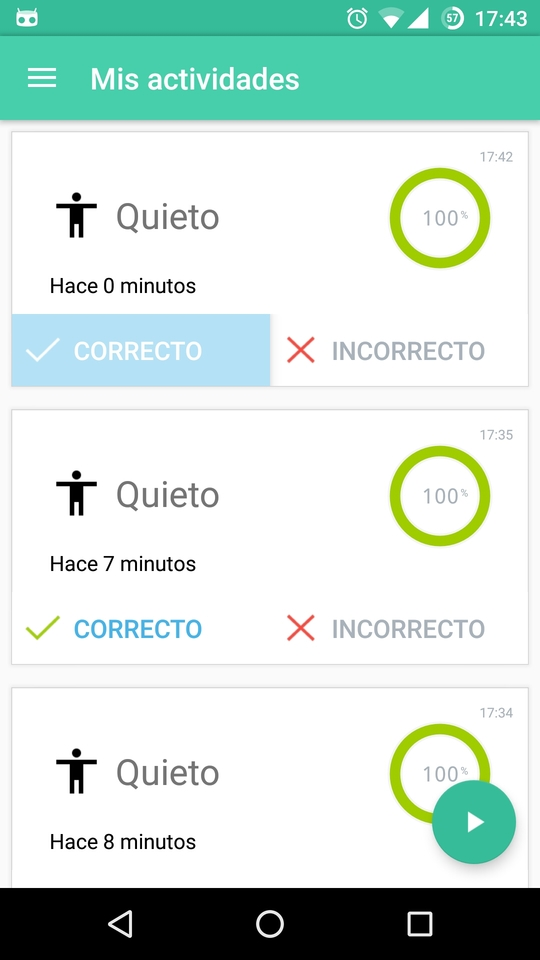
\includegraphics[width=0.33\textwidth]{anexos/graphics/act_ok.jpg}}
 & 
    {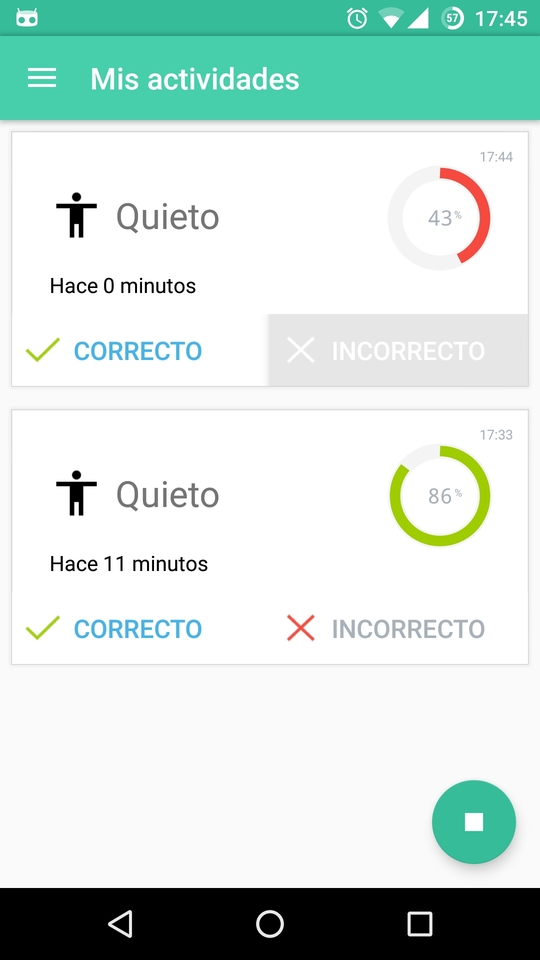
\includegraphics[width=0.33\textwidth]{anexos/graphics/act_nook.jpg}}
 & 
    {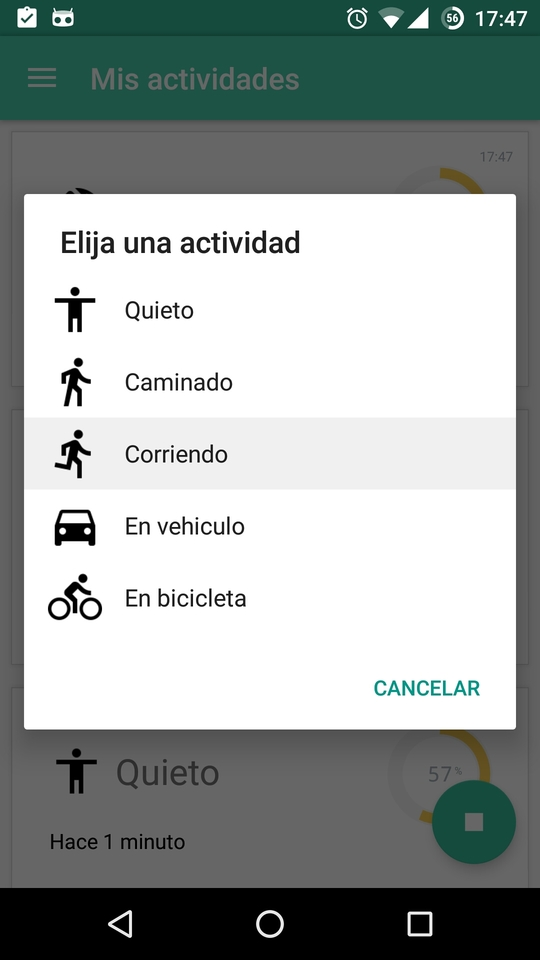
\includegraphics[width=0.33\textwidth]{anexos/graphics/act_feed2.jpg}}
\\
\end{tabular}
\end{table}


Adicionalmente puede ocurrir que no se detecte ninguna actividad.
\begin{quote}
\begin{description}
\item[{Actividad No reconocida}] \leavevmode
El servicio no pudo detectar la activdad física, marcala como incorrecta y proveer la retroalimentación
con la actividad adecuada

\end{description}
\end{quote}

\begin{table}[!htbp]
\begin{tabular}{ll}
\textsf{\relax 
Marcar incorrecto (1)
} & \textsf{\relax 
Responder (3)
}\\
    {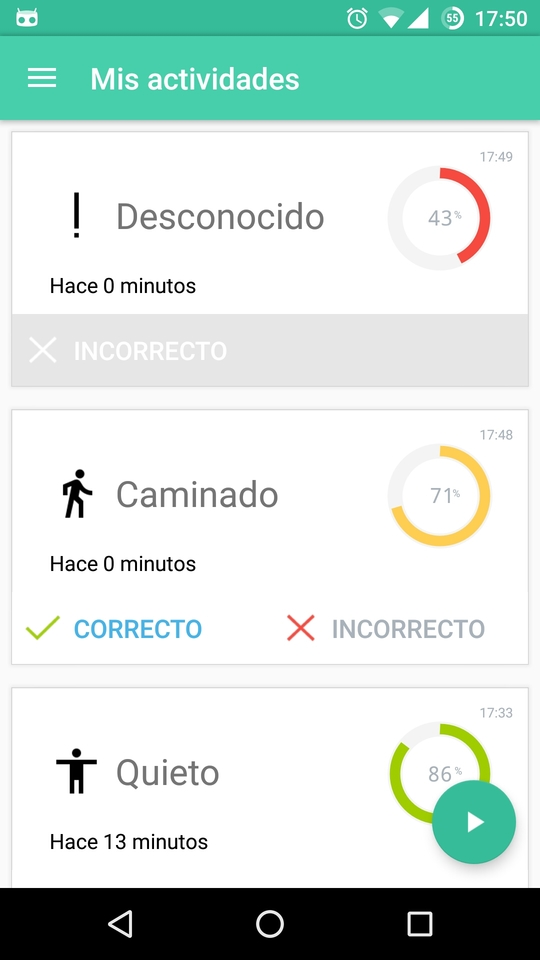
\includegraphics[width=0.33\textwidth]{anexos/graphics/act_nook_unk.jpg}}
 & 
    {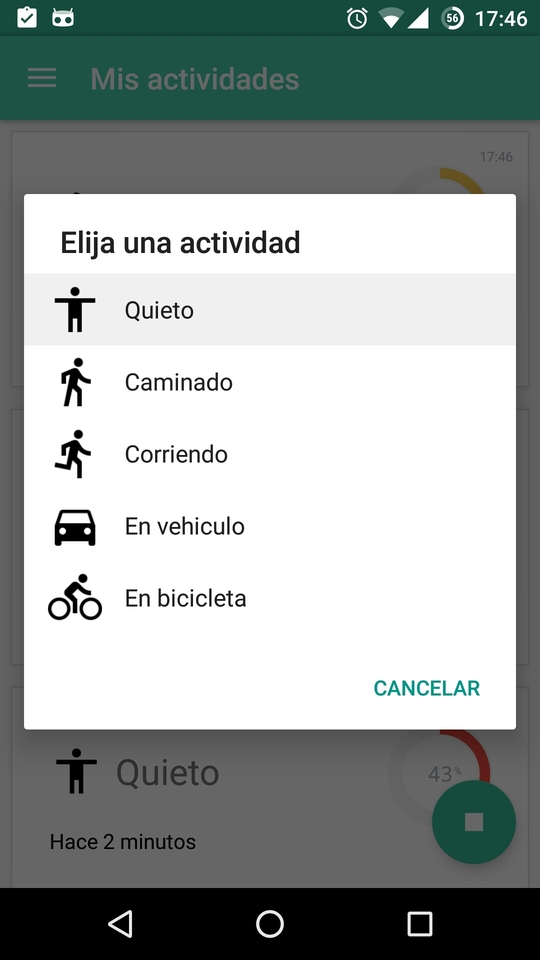
\includegraphics[width=0.33\textwidth]{anexos/graphics/act_feed.jpg}}
\\
\end{tabular}
\end{table}


\subsection{Configuración Adicional}
\label{config_adic:configuracion-adicional}\label{config_adic:har-conf-advanced}\label{config_adic::doc}

\subsubsection{Activar/Desactivar Servicio}
\label{config_adic:activar-desactivar-servicio}
Desde la barra de menú se puede activar y desactivar el servicio de reconocimiento. Presiona el botón
de acción para elegir ambas opciones.

\begin{table}[!htbp]
\begin{tabular}{lll}
\textsf{\relax 
Desactivar Servicio
} & \textsf{\relax 
Activar el Servicio
} & \textsf{\relax 
Servicio Activado
}\\
    {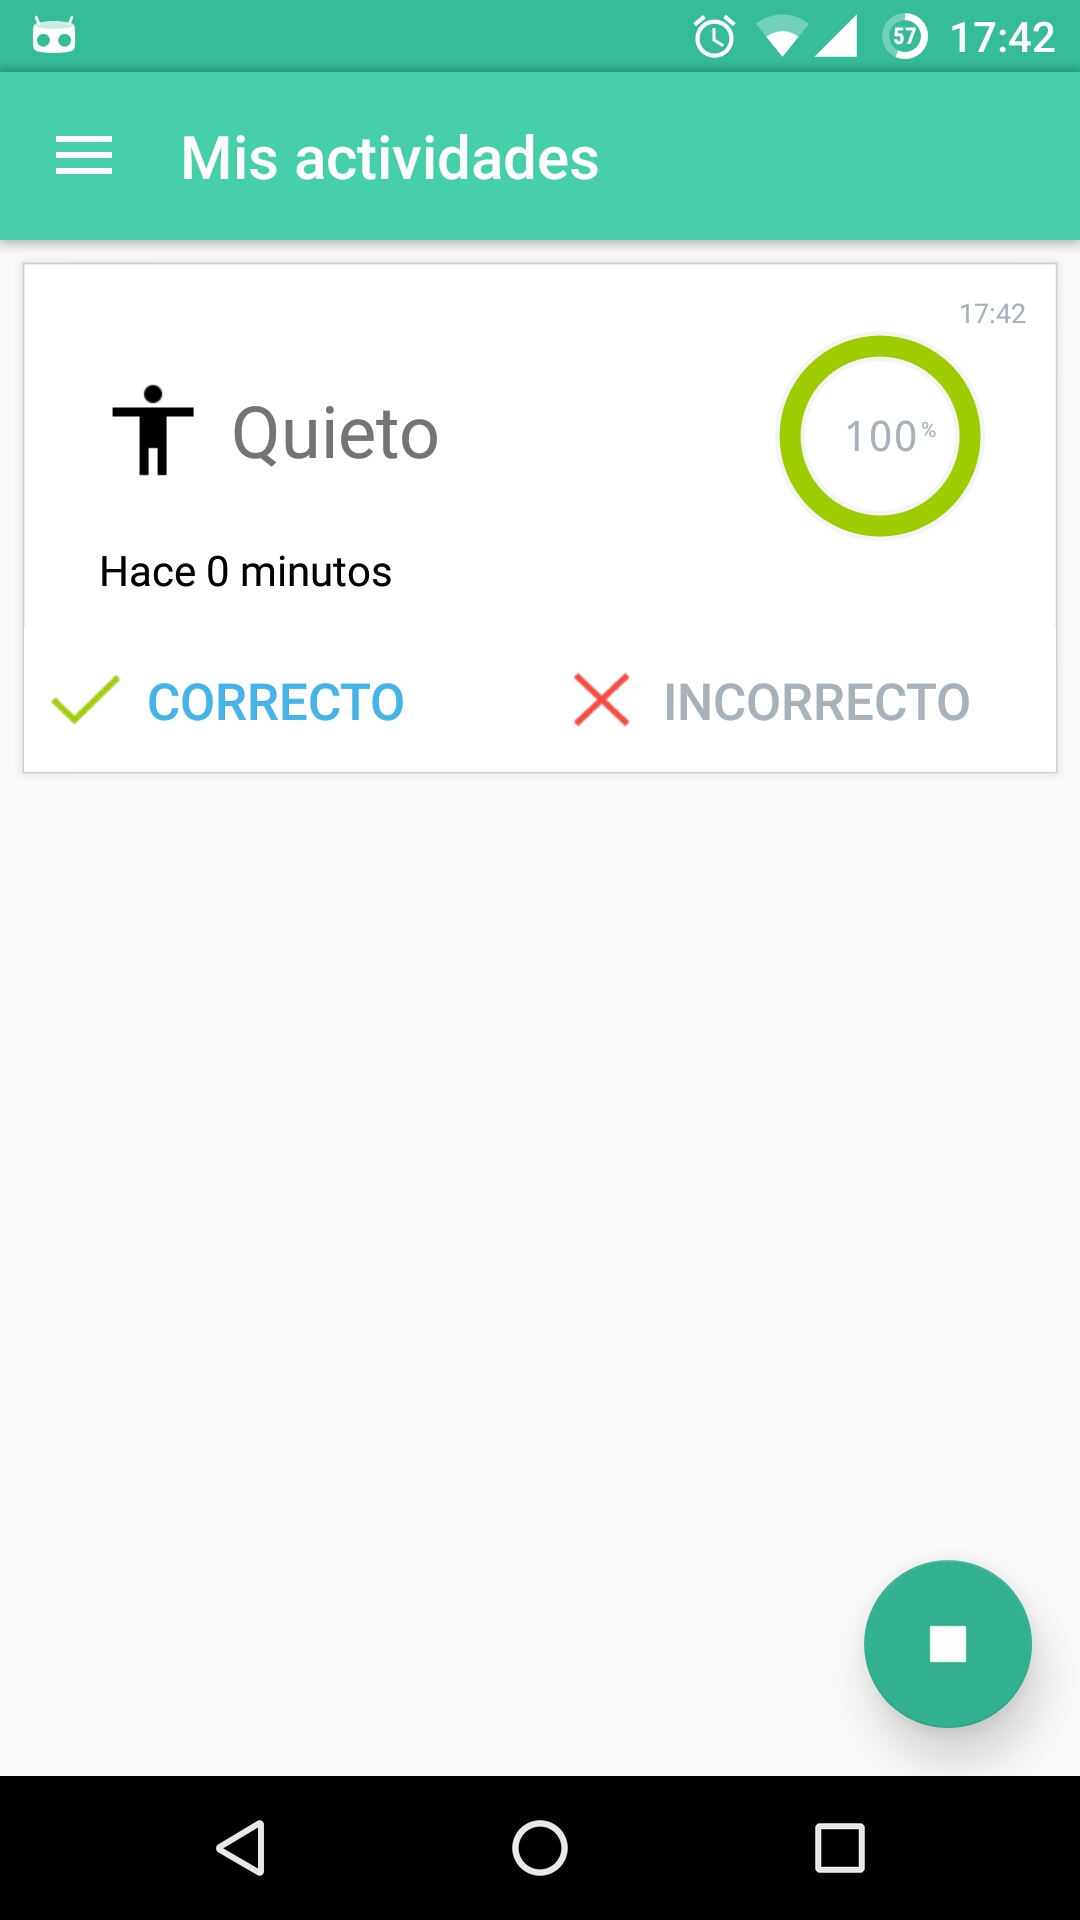
\includegraphics[width=0.33\textwidth]{anexos/graphics/disable_serv.jpg}}
 & 
    {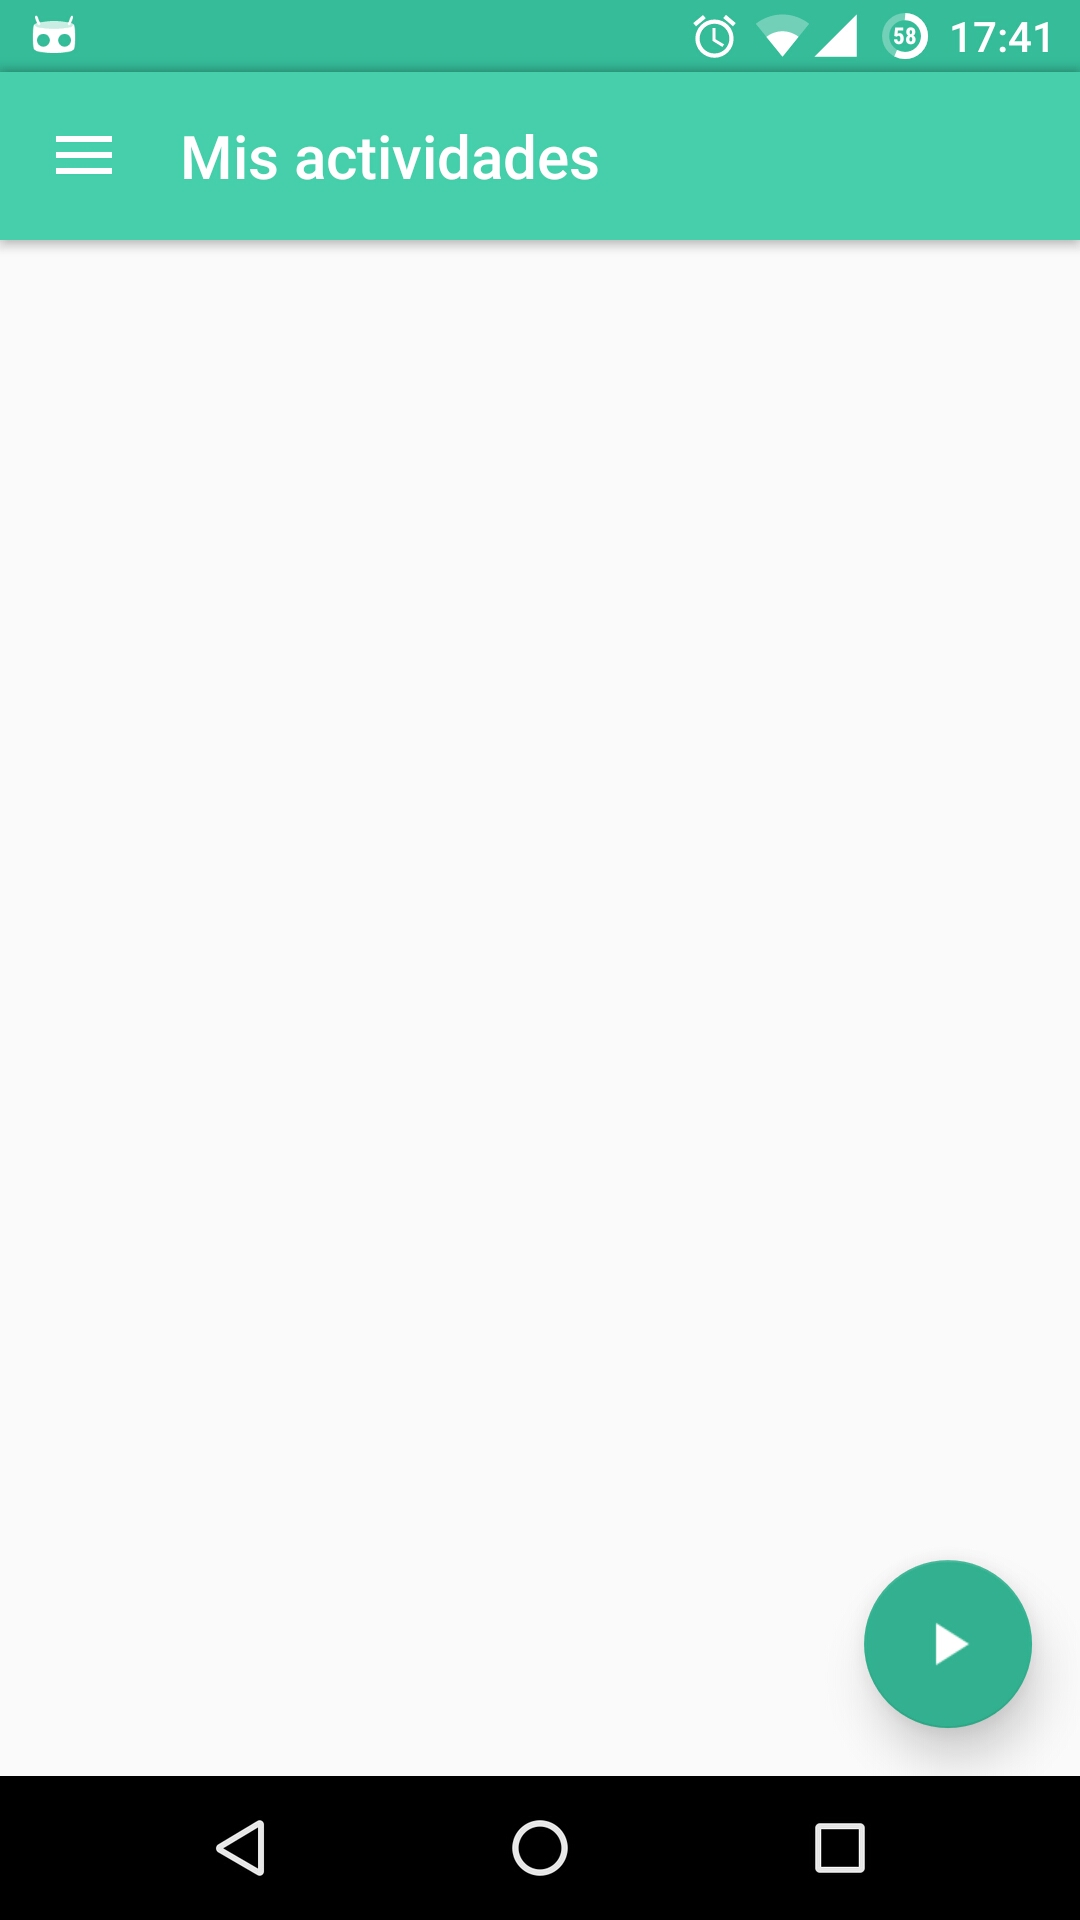
\includegraphics[width=0.33\textwidth]{anexos/graphics/enable_serv.jpg}}
 & 
    {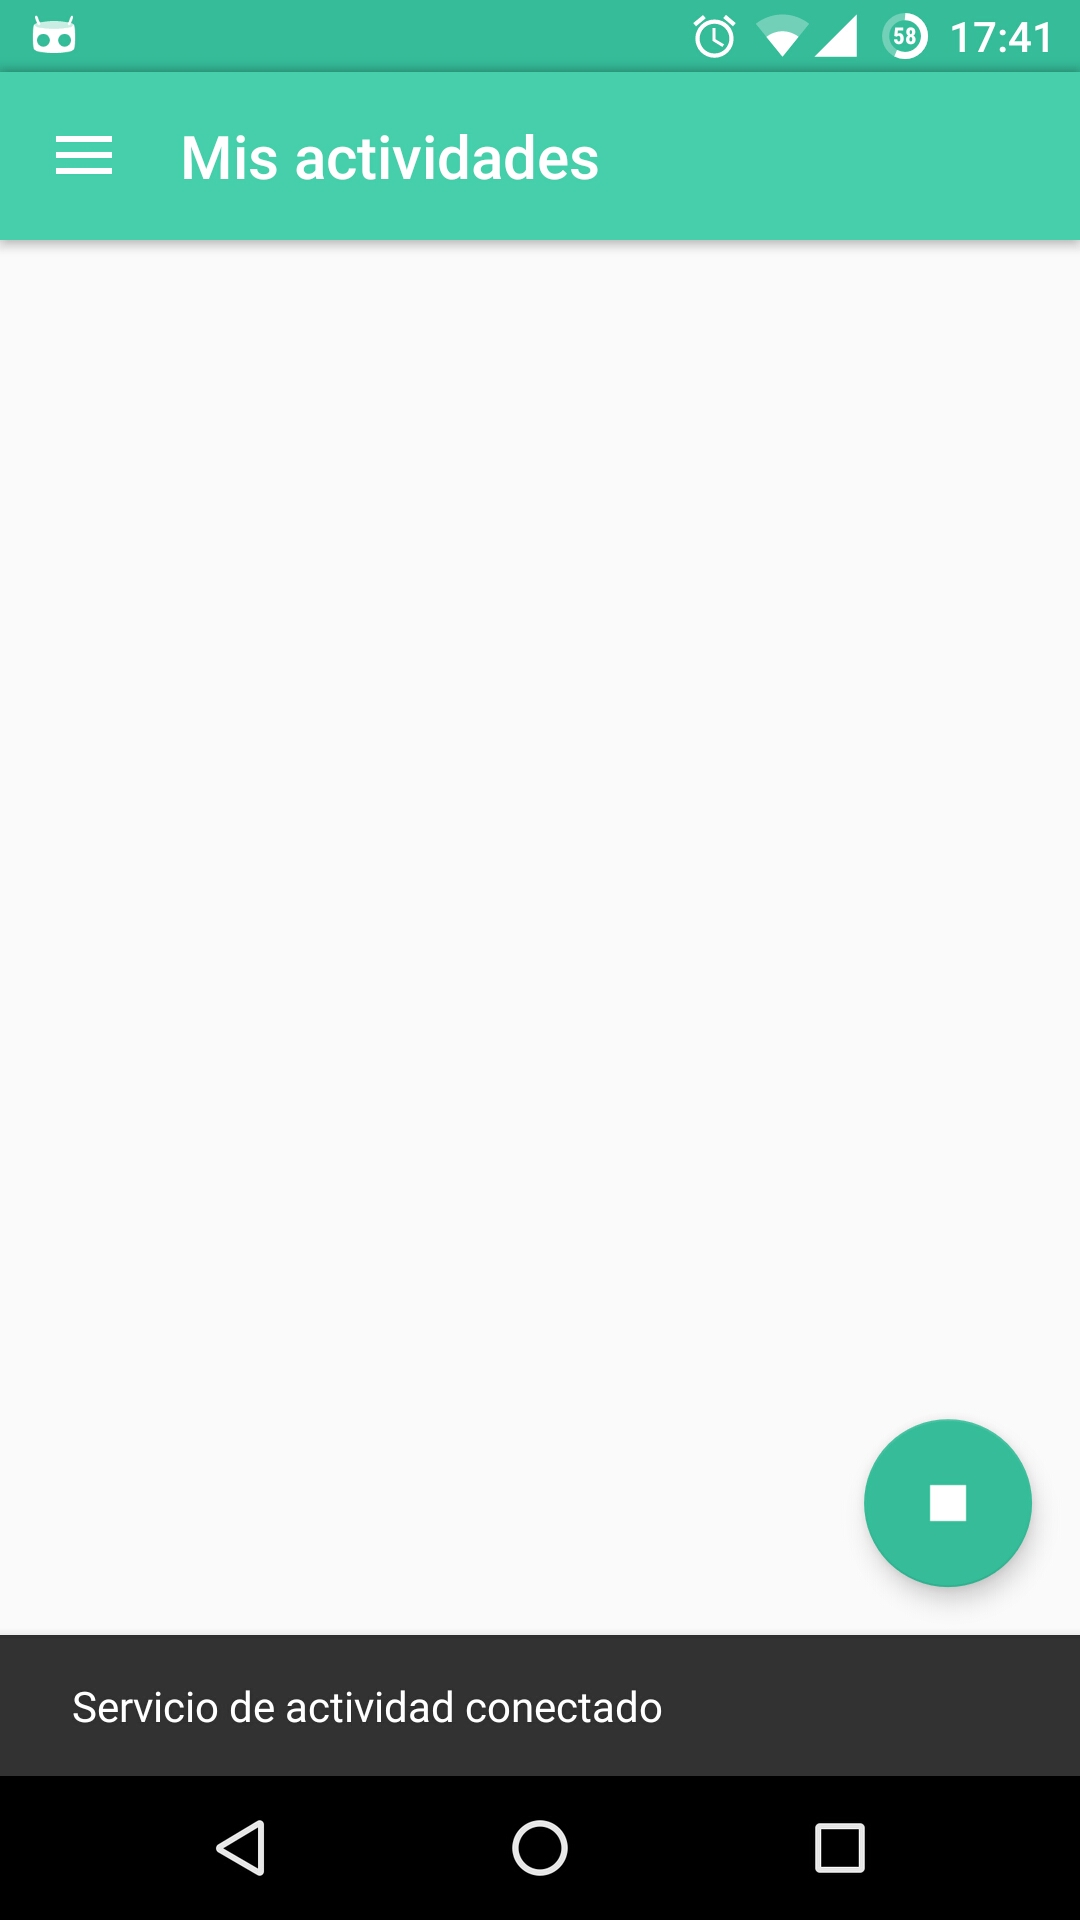
\includegraphics[width=0.33\textwidth]{anexos/graphics/enabled_serv.jpg}}
\\
\end{tabular}
\end{table}


\subsubsection{Configuración}
\label{config_adic:configuracion}
Para acceder a la configuración desde la aplicación accedé al \code{Menu \textgreater{} Configuración}.
\begin{figure}[!htbp]
\centering
    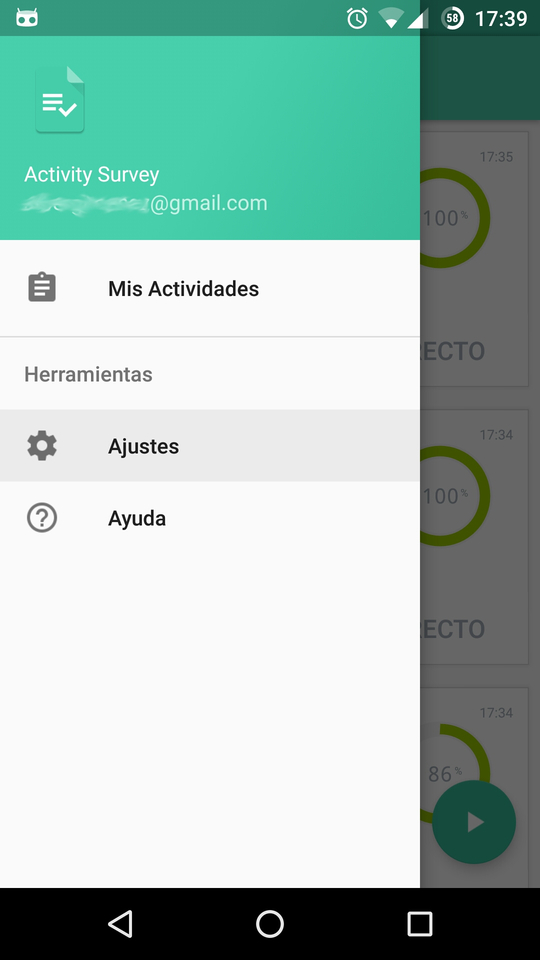
\includegraphics[width=0.4\textwidth]{anexos/graphics/mnu_config.jpg}
\caption{Acceso a la configuración}\label{config_adic:id1}\end{figure}

En esta actividad muestra el detalle de los datos enviados al servidor de encuesta además de las opciones
de configuración como:
\begin{figure}[!htbp]
    \centering
    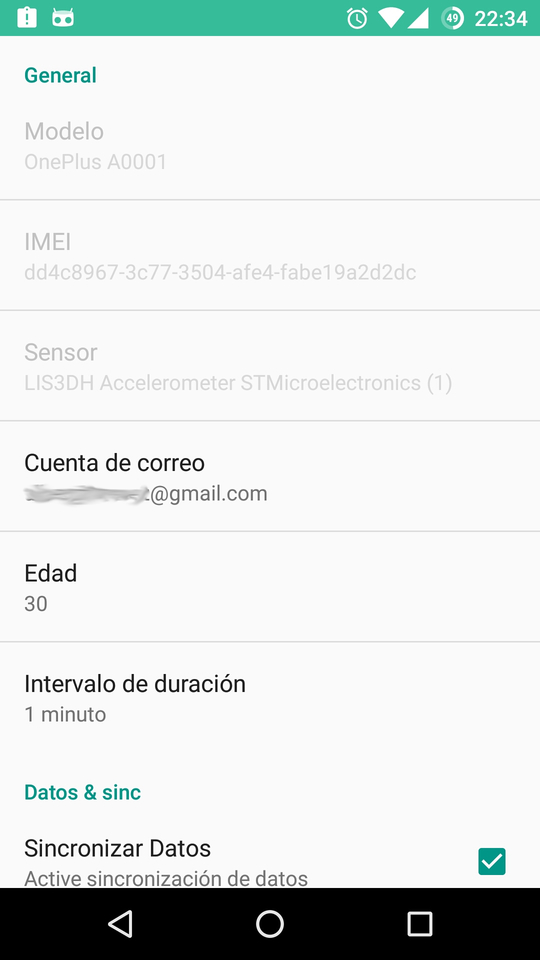
\includegraphics[width=0.4\textwidth]{anexos/graphics/conf_gral.jpg}
\caption{Configuración general}\label{config_adic:id2}\end{figure}


\paragraph{Correo y Edad}
\label{config_adic:correo-y-edad}
Para cambiar la configuración inicial del correo y edad accede las opciones.

\begin{table}[!htbp]
\begin{tabulary}{ll}
\textsf{\relax 
Cambiar correo
} & \textsf{\relax 
Cambiar edad
}\\
    {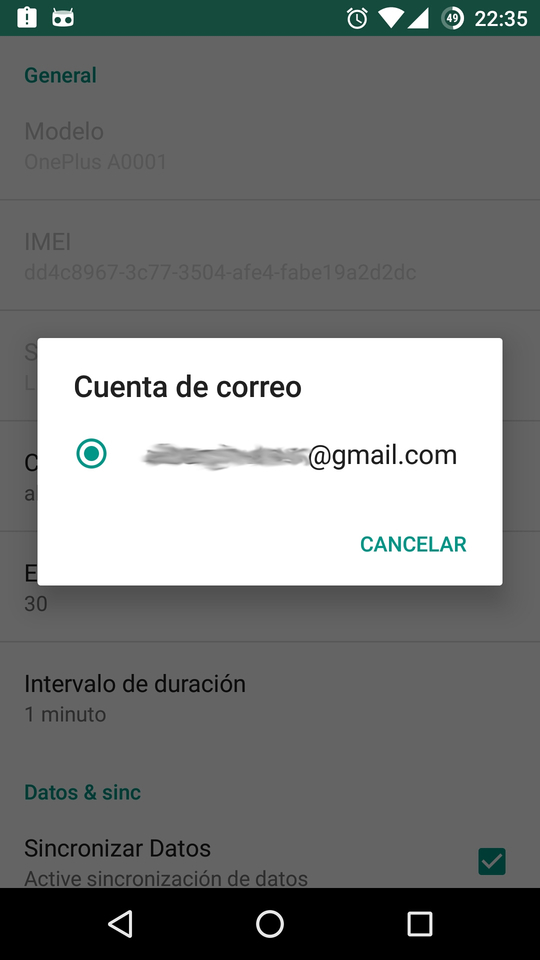
\includegraphics[width=0.33\textwidth]{anexos/graphics/conf_mail.jpg}}
 & 
    {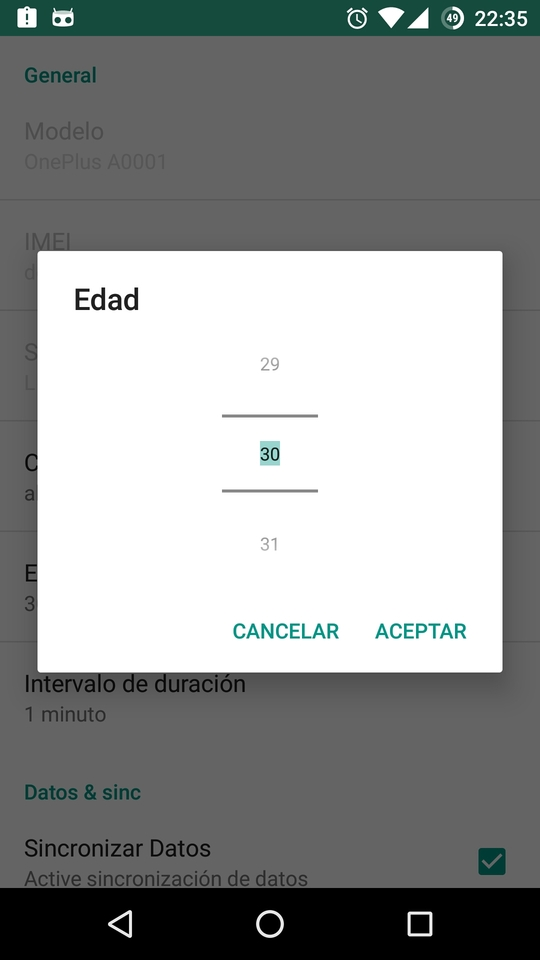
\includegraphics[width=0.33\textwidth]{anexos/graphics/conf_age.jpg}}
\\
\end{tabular}
\end{table}

\paragraph{Intervalo}
\label{config_adic:intervalo}
Para cambiar la configuración del intervalo accede a la opción.
\begin{figure}[!htbp]
    \centering
    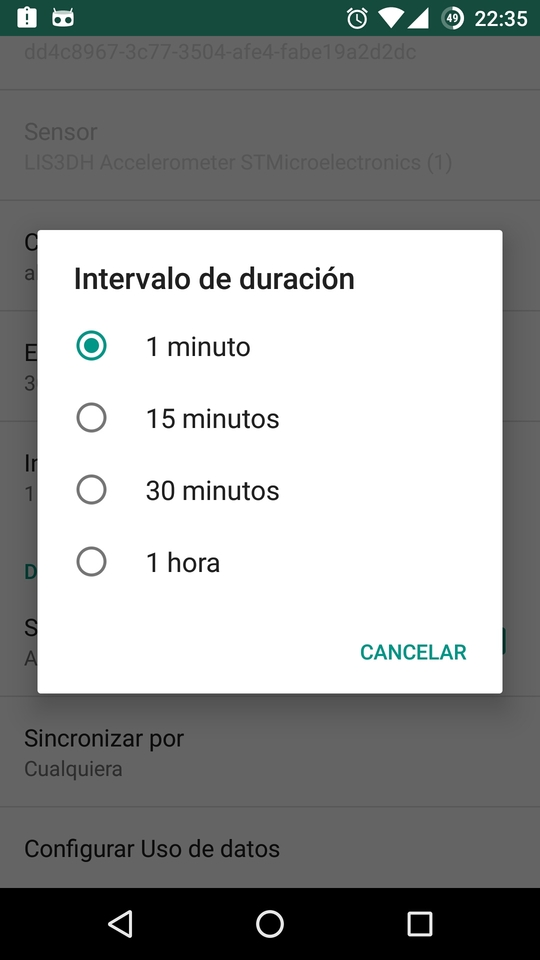
\includegraphics[width=0.4\textwidth]{anexos/graphics/conf_int.jpg}
\caption{Cambiar intervalo}\label{config_adic:id3}\end{figure}


\paragraph{Sincronización de datos}
\label{config_adic:sincronizacion-de-datos}
Para cambiar la manera en que la aplicación envia los datos por WIFI o redes móviles accede a la opción.

\begin{table}[!htbp]
\begin{tabular}{ll}
\textsf{\relax 
Acceso a Sincronizar
} & \textsf{\relax 
Cambiar Sincronizar
}\\
    {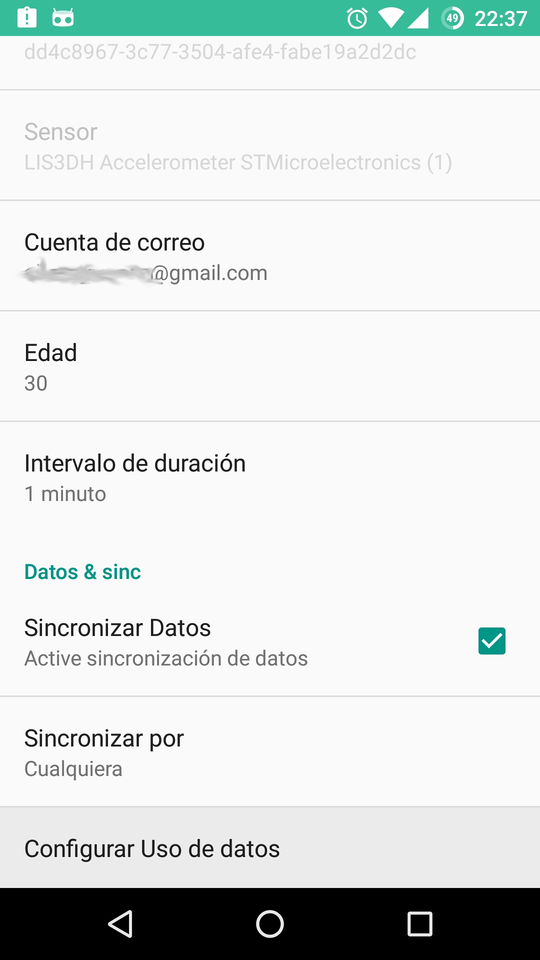
\includegraphics[width=0.33\textwidth]{anexos/graphics/conf_usage.jpg}}
 & 
    {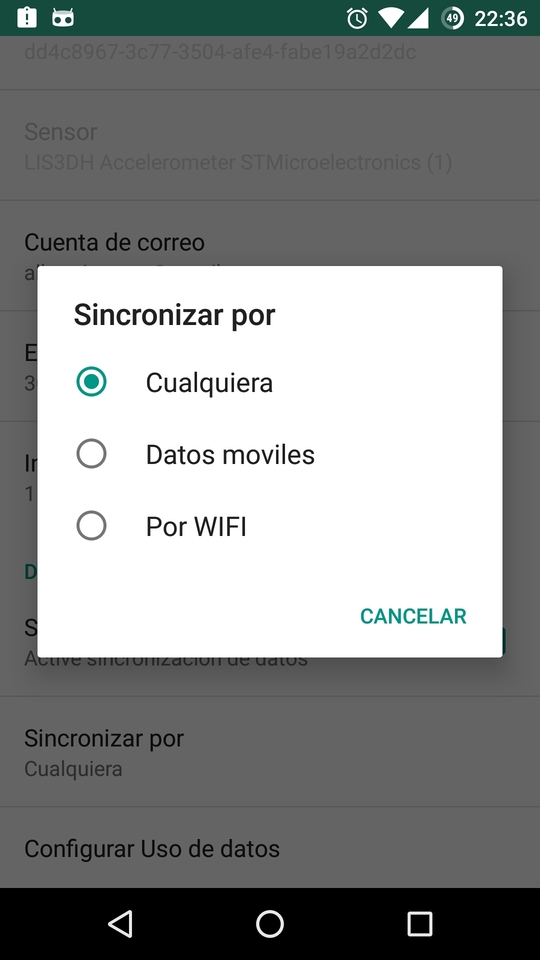
\includegraphics[width=0.33\textwidth]{anexos/graphics/conf_sync.jpg}}
\\
\end{tabular}
\end{table}



\subsubsection{Ayuda}
\label{config_adic:ayuda}
Para acceder a esta página de ayuda desde la aplicación accedé al \code{Menu \textgreater{} Ayuda}.
\begin{figure}[!htbp]
\centering
    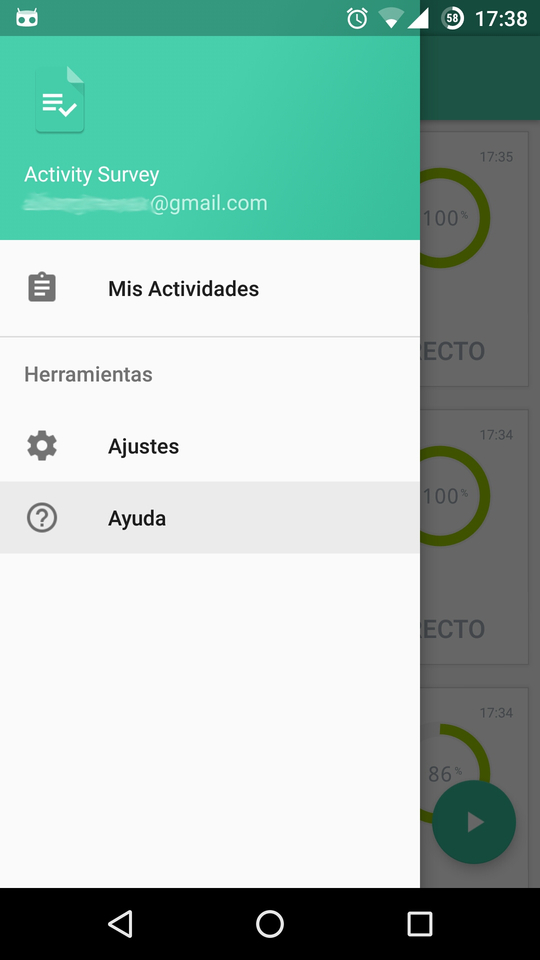
\includegraphics[width=0.4\textwidth]{anexos/graphics/mnu_help.jpg}
\caption{Acceso a la ayuda}\label{config_adic:id4}\end{figure}

\end{description}

